\documentclass[11pt,aspectratio=169]{ctexbeamer}

\usetheme{Berlin}
\useinnertheme{rectangles}
\setbeamertemplate{navigation symbols}{}
\setbeamertemplate{footline}[frame number]

\usepackage{graphicx}
\usepackage{booktabs}
\usepackage{tabularx}
\graphicspath{{img/}}

\definecolor{PrimaryBlue}{HTML}{0E4C92}
\definecolor{AccentOrange}{HTML}{D97B2D}
\definecolor{SoftBg}{HTML}{F4F6F8}
\definecolor{SoftGray}{HTML}{6B7280}
\definecolor{SoftGreen}{HTML}{DCEFE2}
\definecolor{SoftYellow}{HTML}{F7E7B4}

\setbeamercolor{title}{fg=white,bg=PrimaryBlue}
\setbeamercolor{frametitle}{fg=white,bg=PrimaryBlue}
\setbeamercolor{structure}{fg=PrimaryBlue}
\setbeamercolor{block title}{fg=white,bg=PrimaryBlue}
\setbeamercolor{block body}{bg=SoftBg}
\setbeamercolor{alerted text}{fg=AccentOrange}
\setbeamercolor{itemize item}{fg=AccentOrange}
\setbeamercolor{itemize subitem}{fg=PrimaryBlue}

\setbeamertemplate{itemize item}{\small$\blacksquare$}
\setbeamertemplate{itemize subitem}{\small$\blacktriangleright$}

\newcommand{\code}[1]{\texttt{#1}}
\newcommand{\term}[1]{\textbf{\color{PrimaryBlue}#1}}

\AtBeginSection[]{
  \begin{frame}[noframenumbering]{目录}
    \tableofcontents[currentsection,hideallsubsections]
  \end{frame}
}

\title{STM32 USB虚拟串口原理与程序设计}
\subtitle{基于 USB CDC 的通信机制、软件结构与流程设计}
\author{周贤中}
\institute{集成电路学院\\
\vspace{0.5cm}
广东工业大学}
\date{\today}

\begin{document}

\begin{frame}
  \titlepage
\end{frame}

\begin{frame}{目录}
  \tableofcontents
\end{frame}

\section{背景与定位}

\begin{frame}{为什么要学习 USB 虚拟串口}
  \begin{itemize}
    \item 在嵌入式开发中，虚拟串口常用于\term{调试输出}、\term{运行日志}、\term{命令交互}和\term{上位机参数配置}。
    \item 相比传统 UART，USB 直接连接电脑更方便，不必额外准备 USB 转串口模块。
    \item 对教学实验而言，USB 虚拟串口能同时覆盖\term{枚举识别}、\term{双向通信}、\term{字符串处理}和\term{软件分层}等知识点。
    \item 后续实验通常都会建立在这套理论之上：先让电脑识别出 \code{COM} 口，再完成命令收发与业务逻辑。
  \end{itemize}
\end{frame}

\begin{frame}{从传统 UART 串口说起}
  \small
  \begin{columns}[T,onlytextwidth]
    \column{0.58\textwidth}
    \begin{block}{UART 的核心特点}
      \begin{itemize}
        \item 通过 \code{TX}/\code{RX} 两根信号线进行异步通信
        \item 依赖波特率、数据位、校验位、停止位等串口参数
        \item 常见配置写作 \code{115200 8N1}
        \item 其中 \code{115200} 表示波特率，\code{8} 表示 8 位数据位，\code{N} 表示无校验，\code{1} 表示 1 位停止位
        \item 数据按\term{位时序}逐位发送
      \end{itemize}
    \end{block}

    \column{0.38\textwidth}
    \begin{alertblock}{补充说明}
      UART 是\term{异步通信}，没有单独的时钟线，所以通信双方必须事先约定这些参数。
    \end{alertblock}

    \begin{block}{8N1 的最小帧结构}
      典型一帧可理解为：
      \begin{center}
        \code{1起始位 + 8数据位 + 0校验位 + 1停止位}
      \end{center}
      因而发送 1 字节有效数据，线路上通常需要传输 10 bit。
    \end{block}
  \end{columns}
\end{frame}

\begin{frame}{UART 与 USB 虚拟串口的本质区别}
  \small
  \begin{tabularx}{\textwidth}{>{\raggedright\arraybackslash}p{2.8cm}XX}
    \toprule
    对比项 & 传统 UART 串口 & USB 虚拟串口 \\
    \midrule
    物理基础 & 串口外设 + \code{TX/RX} 引脚 & USB 外设 + \code{D+}/\code{D-} 差分线 \\
    通信单位 & 串行位流与帧格式 & USB 数据包 \\
    建链方式 & 直接连线即可通信 & 先枚举，再加载驱动，最后才能通信 \\
    电脑侧表现 & 真正的串口硬件或 USB 转串口芯片映射而来 & USB CDC 驱动在操作系统中创建出的 \code{COM} 接口 \\
    上层使用方式 & 串口助手打开端口收发文本 & 串口助手同样打开端口，但底层已变成 USB \\
    \bottomrule
  \end{tabularx}

  \vspace{0.5em}
  \alert{结论：}“虚拟串口”是\term{接口层面的相似}，不是\term{底层协议完全相同}。
\end{frame}

\section{USB 通信基础}

\begin{frame}{USB 的基本思想}
  \begin{itemize}
    \item USB 是 \term{Universal Serial Bus}，即通用串行总线。
    \item 它不是简单的一根数据线，而是一整套\term{总线协议 + 供电机制 + 枚举机制 + 类规范}。
    \item USB 系统强调\term{即插即用}：设备接入后，主机会主动识别其类型并加载相应驱动。
    \item 对本课程的 STM32 场景来说，开发板扮演 \term{Device}，电脑扮演 \term{Host}。
  \end{itemize}
\end{frame}

\begin{frame}{USB 中的 Host 与 Device}
  \begin{columns}[T,onlytextwidth]
    \column{0.38\textwidth}
    \begin{block}{USB 的主从关系}
      \begin{itemize}
        \item \term{Host}（主机）负责供电、枚举、调度和发起通信
        \item \term{Device}（设备）负责响应主机请求，按协议提供功能
        \item \term{Hub}（集线器）用于扩展主机可连接的 USB 设备数量
        \item 总线访问权由主机掌握，设备不能像 UART 一样主动“抢线”
      \end{itemize}
    \end{block}

    \column{0.56\textwidth}
    \centering
    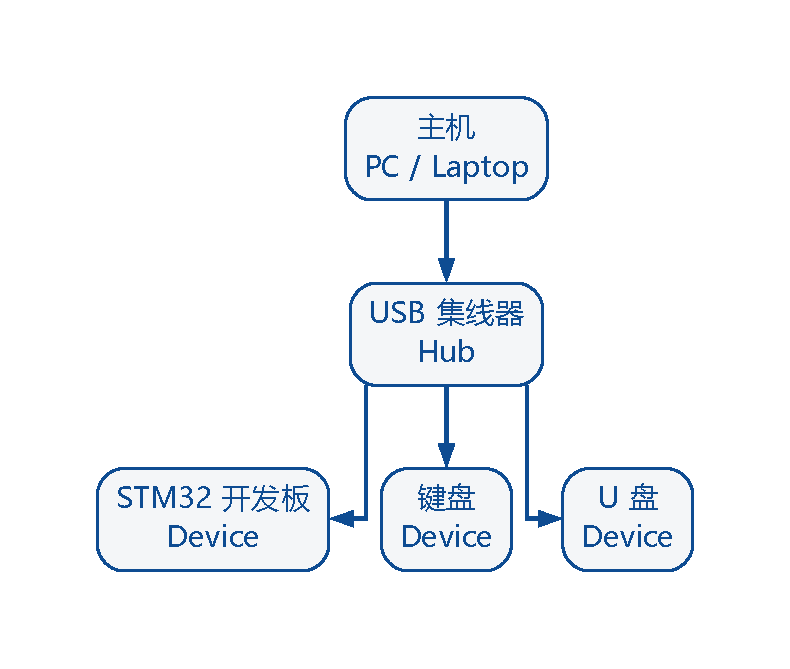
\includegraphics[width=\linewidth,height=0.6\textheight,keepaspectratio]{host_device.pdf}

    \vspace{0.3em}
    \scriptsize
    图中展示的是“一台主机通过集线器连接多个设备”的典型拓扑。若只连接一块 STM32 开发板，也可以不经过外置 Hub，直接与主机相连。
  \end{columns}
\end{frame}

\begin{frame}{USB 设备的逻辑结构}
  \begin{columns}[T,onlytextwidth]
    \column{0.4\textwidth}
    \begin{itemize}
      \item \term{Device}：整个 USB 设备。
      \item \term{Configuration}：设备的一组工作配置。
      \item \term{Interface}：某一类功能接口，例如控制接口、数据接口。
      \item \term{Endpoint}：真正承载数据传输的端点。
    \end{itemize}
    \vspace{0.4em}
    \begin{alertblock}{理解重点}
      主机不是直接面对“某个函数”，而是通过配置、接口和端点来理解设备能力。
    \end{alertblock}

    \column{0.55\textwidth}
    \centering
    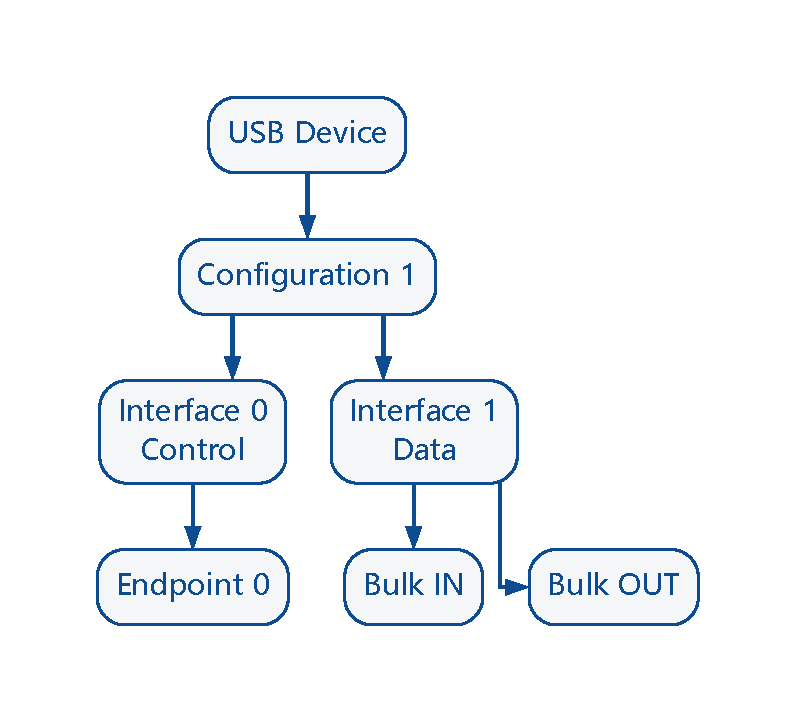
\includegraphics[width=\linewidth]{usb_device_structure.pdf}
  \end{columns}
\end{frame}

\begin{frame}{Descriptor：主机为什么能识别设备}
  \small
  \begin{itemize}
    \item USB 设备具备\term{自描述}能力，主机会主动读取各种描述符来理解设备。
    \item 常见描述符包括：
      \begin{itemize}
        \item \term{设备描述符}：厂商 ID、产品 ID、USB 版本等
        \item \term{配置描述符}：设备有哪些配置
        \item \term{接口描述符}：每个接口属于什么类
        \item \term{端点描述符}：每个端点的方向、类型和大小
        \item \term{字符串描述符}：产品名、厂商名等可读文本
      \end{itemize}
    \item 主机之所以知道“这是一个 CDC 设备”，本质上就是从这些描述符中读出来的。
  \end{itemize}
\end{frame}

\begin{frame}{USB 的四种传输类型}
  \small
  \begin{tabularx}{\textwidth}{>{\raggedright\arraybackslash}p{2.4cm}XX}
    \toprule
    传输类型 & 特点 & 常见用途 \\
    \midrule
    Control & 所有 USB 设备必须支持，主要用于枚举、配置和控制命令 & 读取描述符、设置地址、标准请求 \\
    Bulk & 强调数据正确性，允许重传，但不保证固定实时性 & 虚拟串口、U 盘、大块数据传输 \\
    Interrupt & 适合小数据量、周期性查询，延迟通常较小 & 鼠标、键盘、状态上报 \\
    Isochronous & 强调时间连续性，不强调重传可靠性 & 音频、视频流 \\
    \bottomrule
  \end{tabularx}

  \vspace{0.4em}
  \alert{CDC 虚拟串口通常主要依赖 \code{Control} 和 \code{Bulk}。}
\end{frame}

\begin{frame}{USB 枚举过程}
  \centering
  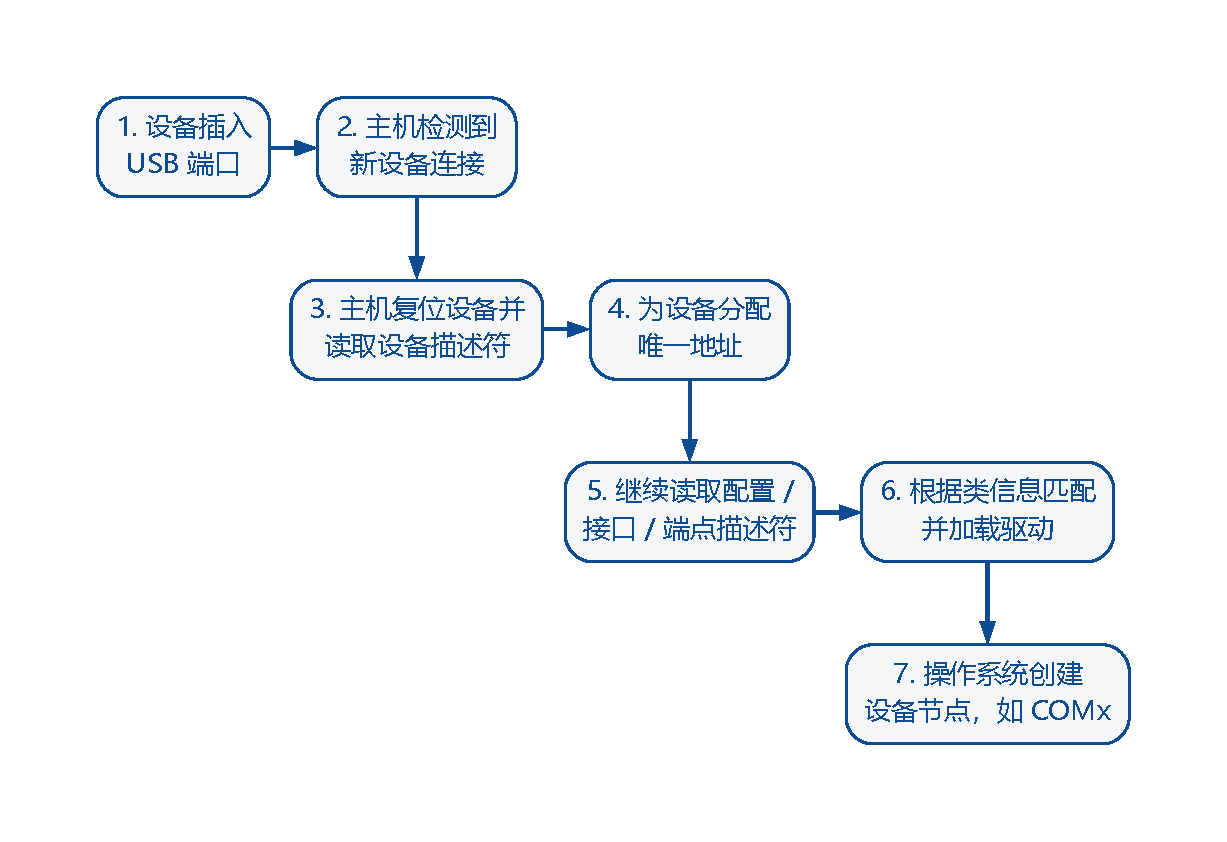
\includegraphics[width=0.9\linewidth,height=0.8\textheight,keepaspectratio]{usb_enumeration.pdf}
\end{frame}

\section{CDC 虚拟串口原理}

\begin{frame}{USB 设备类与 CDC 的定位}
  \begin{itemize}
    \item 为了让主机快速识别设备用途，USB 规范定义了不同的\term{设备类}。
    \item 常见类包括：\code{HID}、\code{MSC}、\code{CDC}、\code{Audio}、\code{Video}。
    \item \term{CDC} 即 \term{Communication Device Class}，原本用于通信类设备。
    \item 在嵌入式开发中，CDC 最常见的应用就是实现\term{虚拟串口}。
  \end{itemize}
\end{frame}

\begin{frame}{为什么 CDC 能成为“虚拟串口”}
  \begin{columns}[T]
    \column{0.58\textwidth}
    \begin{itemize}
      \item 操作系统提供了与 CDC 兼容的驱动模型。
      \item 驱动会把 USB CDC 设备\term{抽象}成一个串口设备接口。
      \item 因此应用程序可以像访问普通串口一样打开 \code{COMx} 并收发数据。
      \item 也就是说：\term{上层像串口，底层是 USB 包传输。}
    \end{itemize}

    \column{0.38\textwidth}
    \begin{block}{常见术语}
      \begin{itemize}
        \item \code{VCP}\\Virtual COM Port
        \item \code{CDC ACM}\\Abstract Control Model
      \end{itemize}
    \end{block}
  \end{columns}
\end{frame}

\begin{frame}{电脑上的 COM 口到底从哪里来}
  \begin{block}{容易混淆的地方}
    当 STM32 作为 USB CDC 设备连接到电脑时，\\
    电脑上出现的 \code{COM} 口并不是“主板多出了一路真实 UART”，\\
    而是\term{操作系统中的驱动层创建出的软件接口}。
  \end{block}

  \vspace{0.5em}
  \begin{itemize}
    \item 串口调试助手看到的是 \code{COMx}
    \item 驱动层处理的是 CDC 设备读写请求
    \item 主机控制器和 USB 总线传输的是 USB 数据包
  \end{itemize}
\end{frame}

\begin{frame}{USB 虚拟串口的数据收发路径}
  \centering
  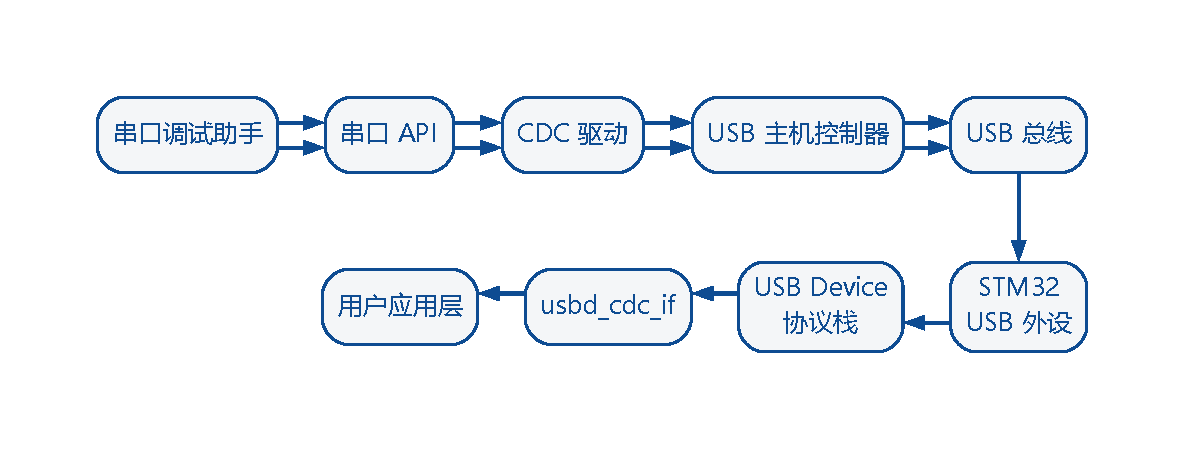
\includegraphics[width=0.92\linewidth,height=0.52\textheight,keepaspectratio]{usb_vcp_data_path.pdf}

  \vspace{0.3em}
  \begin{alertblock}{理解重点}
    串口助手虽然看起来在“直接和串口通信”，实际上中间经过了操作系统驱动和 USB 协议栈。
  \end{alertblock}
\end{frame}

\begin{frame}{虚拟串口与传统 UART：相同点与不同点}
  \small
  \begin{columns}[T]
    \column{0.48\textwidth}
    \begin{block}{相同点}
      \begin{itemize}
        \item 上位机都能打开一个串口接口
        \item 都可以发送文本命令并接收文本响应
        \item 都可用于日志输出和调试终端
      \end{itemize}
    \end{block}

    \column{0.48\textwidth}
    \begin{alertblock}{不同点}
      \begin{itemize}
        \item UART 靠位时序，USB 靠数据包和协议栈
        \item UART 不需要枚举，USB 必须先枚举
        \item UART 常是点对点，USB 由主机统一调度
        \item UART 真正依赖波特率，CDC 通常不依赖串口助手里设置的波特率
      \end{itemize}
    \end{alertblock}
  \end{columns}
\end{frame}

\begin{frame}{为什么串口助手还要设置 115200 8N1}
  \begin{itemize}
    \item 很多上位机软件是按“串口工具”的统一界面设计的，因此仍然要求填写波特率、数据位、校验位和停止位。
    \item 对 USB CDC 虚拟串口而言，这些参数通常\term{不会像传统 UART 那样真正决定底层 USB 传输速率}。
    \item 之所以仍常写成 \code{115200 8N1}，主要是为了：
      \begin{itemize}
        \item 保持软件界面一致
        \item 避免工具因参数为空而无法打开端口
        \item 让实验文档书写格式统一
      \end{itemize}
  \end{itemize}

  \vspace{0.4em}
  \alert{结论：}在 USB CDC 场景下，\code{115200 8N1} 更多是\term{接口兼容信息}，而不是 USB 总线速率配置。
\end{frame}

\section{STM32 中的 USB CDC}

\begin{frame}{STM32 为什么能够实现 USB 虚拟串口}
  \begin{itemize}
    \item 芯片必须具备 \term{USB Device} 外设，能够处理 USB 全速设备通信。
    \item 硬件上要有 \code{D+}/\code{D-} 引脚及相关连线条件。
    \item 软件上需要 USB Device 协议栈和 CDC 类中间件。
    \item 在 STM32CubeMX 中启用 \code{USB Device CDC} 后，系统会生成一套基础框架。
    \item 用户程序则在这套框架上补充发送、接收和命令处理逻辑。
  \end{itemize}
\end{frame}

\begin{frame}{STM32 USB CDC 的软件分层}
  \centering
  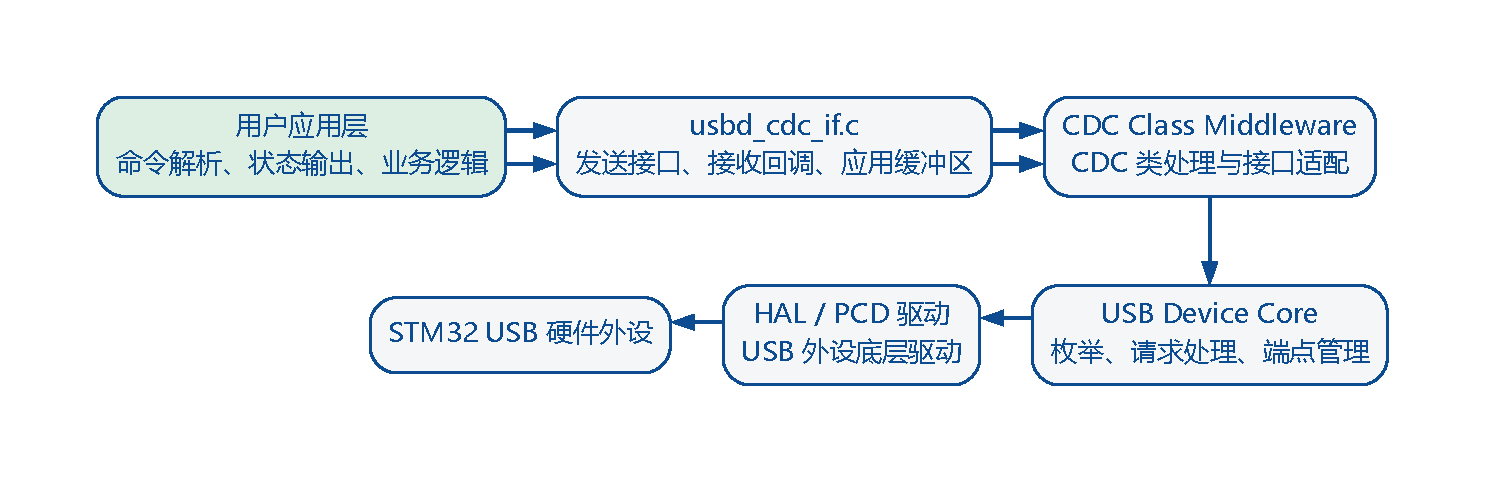
\includegraphics[width=0.92\linewidth,height=0.46\textheight,keepaspectratio]{stm32_usb_stack.pdf}
\end{frame}

\begin{frame}{为什么 USB 时钟必须精确到 48 MHz}
  \begin{itemize}
    \item USB Full Speed 外设对时钟精度要求很高，STM32 的 USB 模块通常需要\term{准确的 48 MHz 时钟}。
    \item 如果时钟来源或分频设置错误，最直接的后果就是：
      \begin{itemize}
        \item 电脑无法识别设备
        \item 能识别但连接不稳定
        \item 数据收发异常或偶发失败
      \end{itemize}
    \item 因此，USB CDC 的问题排查往往首先要检查时钟树，而不是一上来就怀疑字符串处理代码。
  \end{itemize}

  \vspace{0.4em}
  \begin{alertblock}{工程结论}
    “电脑看不到 \code{COM} 口”时，\term{48 MHz} 配置错误通常是首要检查项之一。
  \end{alertblock}
\end{frame}

\begin{frame}{STM32 USB CDC 的发送机制}
  \small
  \begin{itemize}
    \item 用户层通常通过 \code{CDC\_Transmit\_FS()} 或其封装函数发送数据。
    \item 发送请求不会保证每次都立即成功，因为底层端点可能仍在发送上一包数据。
    \item 当接口返回 \code{USBD\_BUSY} 时，说明当前发送资源尚未空闲。
    \item 因而一个稳定的发送函数一般要考虑：
      \begin{itemize}
        \item 是否需要短时间重试
        \item 是否设置超时，避免长时间卡死
        \item 是否在应用层实现发送队列
      \end{itemize}
  \end{itemize}

  \begin{block}{设计启示}
    USB CDC 的发送不是“写一行函数就万事大吉”，而是要把\term{忙状态}当作正常情况来处理。
  \end{block}
\end{frame}

\begin{frame}{STM32 USB CDC 的接收机制}
  \small
  \begin{itemize}
    \item 主机发送 USB 数据包后，STM32 的 USB 外设和协议栈会接收数据并回调到 CDC 接口层。
    \item 在典型工程中，\code{CDC\_Receive\_FS()} 负责：
      \begin{itemize}
        \item 读取 \code{Buf} 与 \code{Len}
        \item 将数据复制到应用层缓冲区
        \item 记录接收长度
        \item 置位“收到新数据”的标志
        \item 重新开启下一次接收
      \end{itemize}
    \item 真正的命令解析、字符串比较和业务处理，通常放在主循环或 RTOS 任务中完成。
  \end{itemize}
\end{frame}

\begin{frame}{为什么不建议在接收回调里做复杂业务}
  \begin{columns}[T]
    \column{0.56\textwidth}
    \begin{itemize}
      \item 回调函数应尽量短，优先保证收包链路持续可用。
      \item 如果在回调里直接做复杂字符串处理、格式化输出或耗时逻辑，会导致：
        \begin{itemize}
          \item 回调执行时间变长
          \item 软件结构混乱
          \item 后续扩展困难
          \item 数据连续输入时更容易丢包或处理不及时
        \end{itemize}
      \item 更好的结构是：\term{回调搬运数据，主循环处理业务。}
    \end{itemize}

    \column{0.4\textwidth}
    \begin{alertblock}{设计思想}
      这是一种非常典型的嵌入式软件设计思想：\\[0.3em]
      \textbf{中断/回调收集数据，前台处理复杂逻辑。}
    \end{alertblock}
  \end{columns}
\end{frame}

\begin{frame}{共享数据与同步问题}
  \begin{itemize}
    \item 接收缓冲区、接收长度和接收标志位通常同时被\term{回调函数}与\term{主循环}访问。
    \item 这类变量通常需要考虑：
      \begin{itemize}
        \item 使用 \code{volatile}，防止编译器错误优化
        \item 拷贝共享缓冲区时进入临界区，避免读写冲突
        \item 控制缓冲区长度，防止越界
      \end{itemize}
    \item 如果忽略这些同步问题，程序可能表现为：
      \begin{itemize}
        \item 偶发解析错误
        \item 字符串截断
        \item 标志位状态异常
      \end{itemize}
  \end{itemize}
\end{frame}

\section{程序设计要点与流程图}

\begin{frame}{程序设计的总体思路}
  \begin{enumerate}
    \item 先完成系统时钟、GPIO、USB Device 和 CDC 中间件初始化。
    \item 等待 USB 枚举稳定，再发送欢迎信息或启动提示。
    \item 使用“\term{接收缓冲区 + 长度变量 + 标志位}”构成应用层接收通道。
    \item 在 \code{CDC\_Receive\_FS()} 中只做最小动作：复制数据、记录长度、置位标志、重新开启接收。
    \item 主循环检测标志位后再解析命令、组织响应并调用发送接口。
  \end{enumerate}
\end{frame}

\begin{frame}{STM32 USB 虚拟串口程序设计要点}
  \small
  \begin{itemize}
    \item \term{初始化顺序要清晰}：时钟错误会直接导致设备无法枚举。
    \item \term{发送函数要可恢复}：应考虑 \code{USBD\_BUSY}、超时和重试策略。
    \item \term{接收路径要简单}：优先把数据从底层搬到自己的应用缓冲区。
    \item \term{命令处理要放在主循环}：便于调试、扩展和维护。
    \item \term{字符串处理要谨慎}：注意 \code{\textbackslash r}/\code{\textbackslash n}、结尾 \code{\textbackslash0}、缓冲区上限。
    \item \term{程序要有可观测性}：欢迎信息、状态命令、心跳输出都能显著降低调试难度。
  \end{itemize}
\end{frame}

\begin{frame}{典型模块划分}
  \begin{columns}[T]
    \column{0.48\textwidth}
    \begin{block}{\code{main.c}}
      \begin{itemize}
        \item 系统初始化
        \item 主循环
        \item 周期任务
        \item 调用命令处理函数
      \end{itemize}
    \end{block}

    \column{0.48\textwidth}
    \begin{block}{\code{usbd\_cdc\_if.c}}
      \begin{itemize}
        \item 发送接口封装
        \item 接收回调
        \item 应用共享缓冲区
        \item 与 USB Device 栈对接
      \end{itemize}
    \end{block}
  \end{columns}

  \vspace{0.5em}
  \begin{alertblock}{模块边界}
    协议栈负责 USB 通信框架，应用层负责“收到什么、如何解释、返回什么”。
  \end{alertblock}
\end{frame}

\begin{frame}{程序总体流程图}
  \centering
  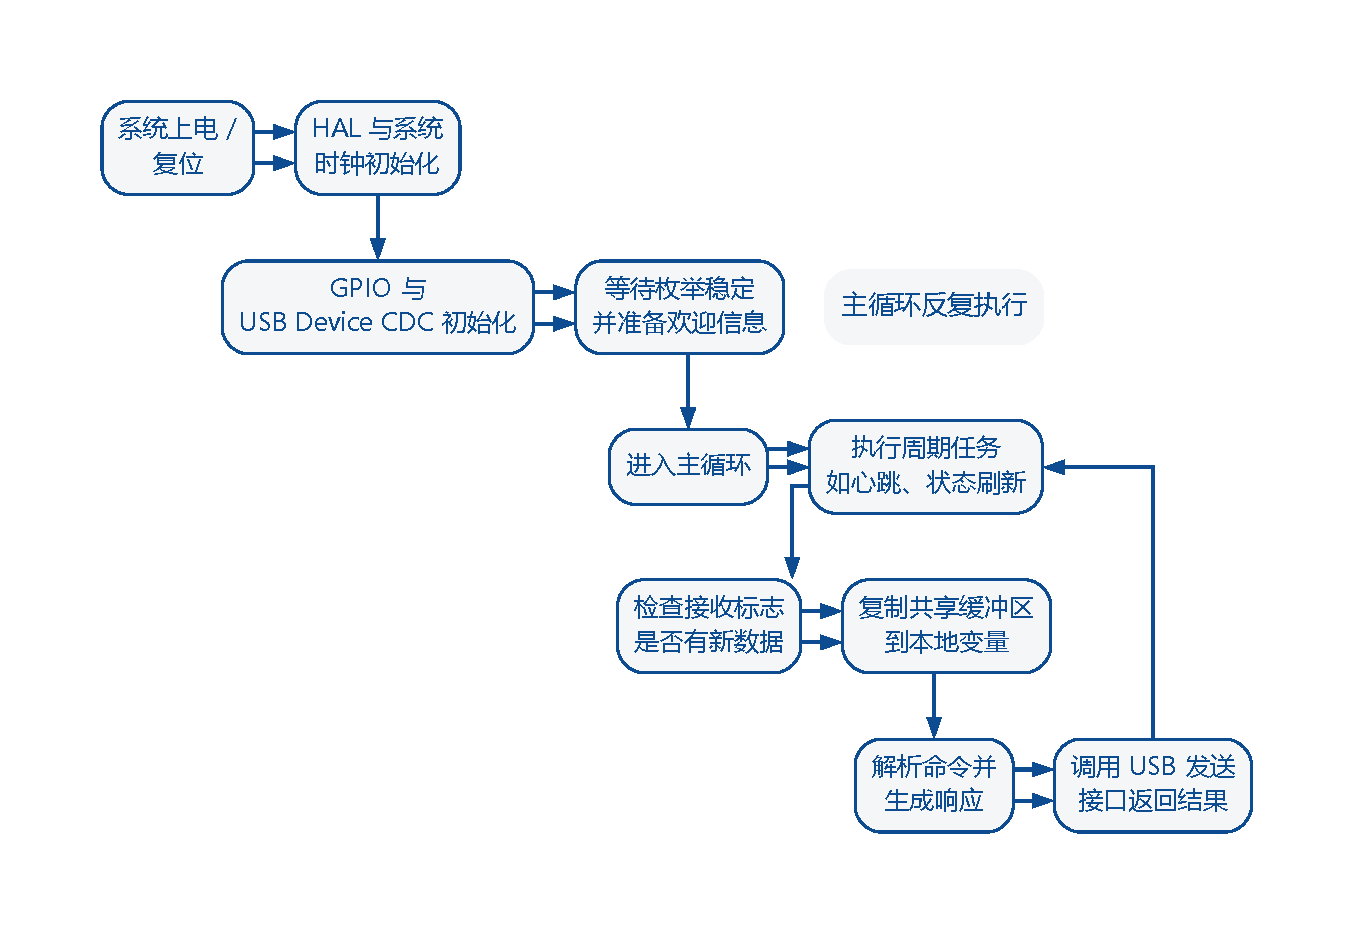
\includegraphics[width=0.82\linewidth,height=\textheight,keepaspectratio]{program_flow.pdf}
\end{frame}

\begin{frame}{接收回调与主循环协作流程图}
  \begin{columns}[T,onlytextwidth]
    \column{0.64\textwidth}
    \centering
    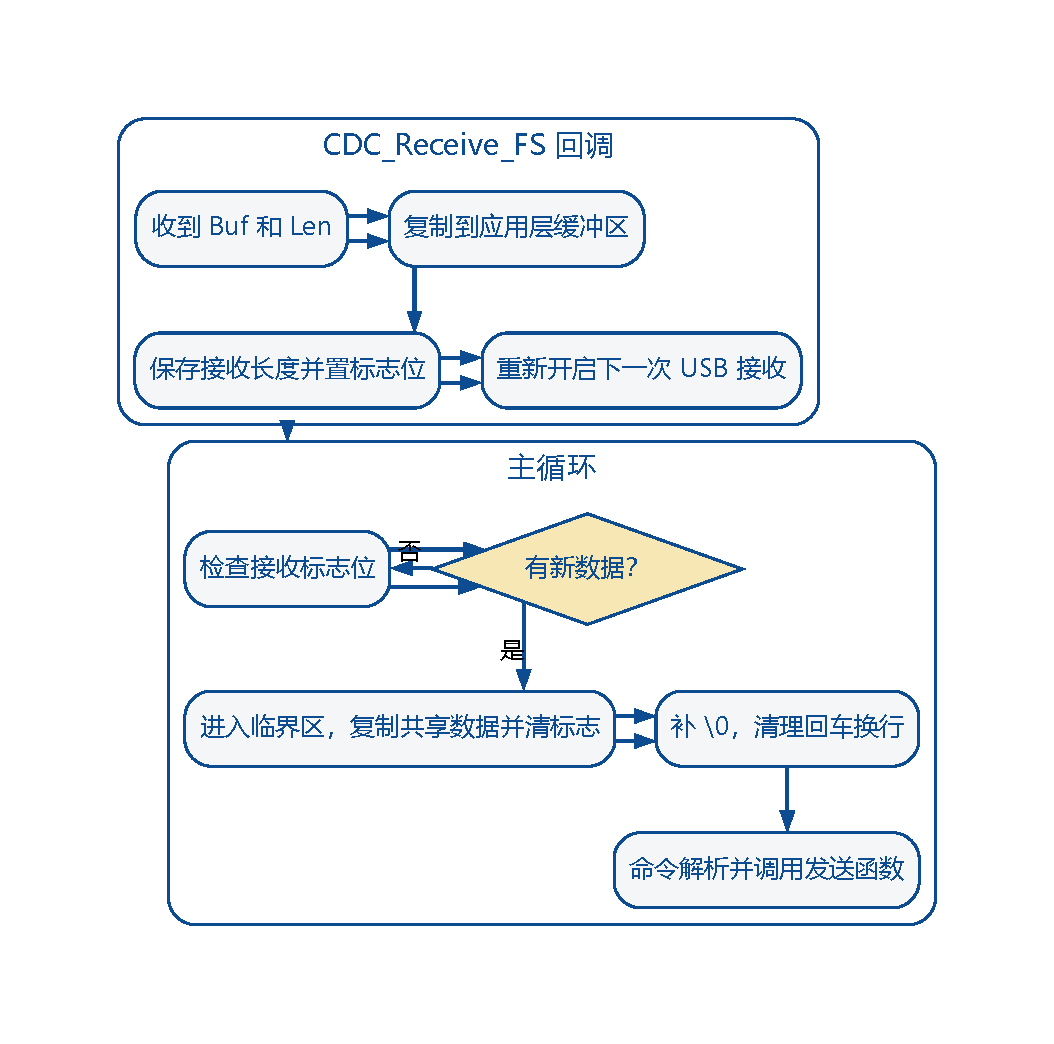
\includegraphics[width=\linewidth,height=0.9\textheight,keepaspectratio]{callback_main_flow.pdf}

    \column{0.32\textwidth}
    \small
    \begin{block}{阅读要点}
      \begin{itemize}
        \item 回调函数负责收包、搬运数据和置位标志
        \item 主循环负责读取共享数据、清标志并处理业务
        \item 虚线表示通过共享缓冲区和标志位完成前后台协作
      \end{itemize}
    \end{block}
  \end{columns}
\end{frame}

\begin{frame}{与后续实验的衔接}
  \begin{itemize}
    \item 后续实验部分并不是重新设计一套程序，而是在本节给出的结构上填入具体代码。
    \item CubeMX 负责生成 \term{USB Device CDC 基础框架}，学生主要补充的是：
      \begin{itemize}
        \item 发送封装函数
        \item 接收回调中的应用层搬运逻辑
        \item 主循环中的命令解析与响应生成
      \end{itemize}
    \item 本节两张流程图可以直接作为实验报告中的\term{程序设计说明}和\term{程序流程图}基础。
  \end{itemize}
\end{frame}

\begin{frame}{总结}
  \begin{itemize}
    \item USB 虚拟串口本质上是\term{USB CDC 设备}，不是底层仍然使用 UART 的“假串口”。
    \item 电脑侧出现的 \code{COM} 口来自\term{驱动抽象}，其前提是枚举、描述符和类匹配都正确。
    \item 对 STM32 而言，理解\term{48 MHz 时钟}、\term{发送忙状态}、\term{接收回调}和\term{主循环协作}是掌握该主题的关键。
    \item 在工程实现上，推荐采用“\term{回调收数据，主循环做业务}”的结构，这也是后续实验的标准基础框架。
  \end{itemize}
\end{frame}

\end{document}
